\documentclass{standalone}
\usepackage{tikz}

\usetikzlibrary{calc}


\begin{document}

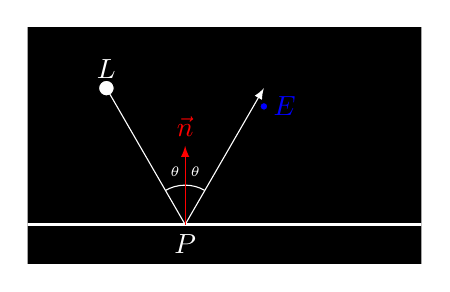
\begin{tikzpicture}
  \path[clip] (-2,-0.5) rectangle (3,2.5);
  \draw[fill=black,black] (-2,-0.5) rectangle (3,2.5);
  \draw[thick,white] (-3,0) -- (4,0);

  \coordinate (hit) at (0,0);
  \coordinate (light) at ($ (hit) + (120:2) $);
  \coordinate (eye) at (1,1.5);
  
  \draw[fill=blue] (eye) circle [radius=0.05cm] node[right,blue] {$E$};
  \draw[fill=white] (light) circle [radius=0.1cm] node [white,above] {$L$};
  \node[anchor=north,white] at (hit) {$P$};
  \draw[white,-latex] (light) -- (hit) -- (60:2);
  \draw[white] (hit) ++(60:0.5) arc[start angle=60,end angle=90,radius=0.5cm] node[above,midway,font=\tiny] {$\theta$};
  \draw[white] (hit) ++(90:0.5) arc[start angle=90,end angle=120,radius=0.5cm] node[above,midway,font=\tiny] {$\theta$};
  \draw[red,-latex] (hit) -- ++(0,1) node[above] {$\vec n$};
\end{tikzpicture}

\end{document}